\documentclass[a4paper,12pt]{scrartcl}

\usepackage[utf8]{inputenc} 
\usepackage[T1]{fontenc}
\usepackage[english]{babel}
\usepackage{amsmath, amssymb,amsfonts}
\usepackage{graphicx}
\usepackage{csquotes}
\usepackage{geometry}
\usepackage{float}
\usepackage{framed, xcolor} 
\usepackage{scrlayer-scrpage}
\usepackage{siunitx}
\usepackage{subcaption}
\usepackage{chemgreek}
\usepackage{chemformula}
\usepackage[bookmarks,colorlinks=true]{hyperref}
\usepackage{booktabs}

% 1. ZUERST DIE VARIABLEN DEFINIEREN
\newcommand{\VERSUCHSDATUM}{March 2, 2026}
\newcommand{\PROTOKOLLDATUM}{\today}
\newcommand{\VerfasserEINS}{Julian Brügger}
\newcommand{\MatNoEINS}{3715444}
\newcommand{\EmailEINS}{st190050@stud.uni-stuttgart.de}
\newcommand{\StudiengangEINS}{B.Sc. Chemie}
\newcommand{\VerfasserZWEI}{Benedict Roßkopf}
\newcommand{\MatNoZWEI}{3718292}
\newcommand{\EmailZWEI}{st188124@stud.uni-stuttgart.de}
\newcommand{\StudiengangZWEI}{B.Sc. Simulation Technology}
\newcommand{\BETREUER}{}
\newcommand{\GRUPPENNR}{Gruppe X} % Darf nicht leer sein, wenn im Header genutzt
\newcommand{\VERSUCHSNR}{1}
\newcommand{\VERSUCHSNAME}{Reaction enthalpies and harmonic vibrational frequencies}

% 2. DANN DAS LAYOUT
\geometry{left = 2.5cm, top = 3cm}
\renewcaptionname{english}{\figurename}{Fig.}
\renewcaptionname{english}{\tablename}{Tab.}

\sisetup{
    detect-weight=true, 
    detect-family=true,
    locale=UK,
    exponent-product = \cdot,
    separate-uncertainty=true,
    per-mode = symbol-or-fraction
}

\DeclareSIUnit{\angstrom}{\text{\AA}}

\hypersetup{
    colorlinks,
    linktocpage,
    citecolor=black,
    filecolor=black,
    linkcolor=black,
    urlcolor=black
}

\setlength{\parindent}{0 mm}
\setlength{\parskip}{2 mm} 

\pagestyle{scrheadings}
\clearpairofpagestyles % Löscht alte Voreinstellungen
\ihead{\VERSUCHSNR} 
\ofoot{\thepage} 

\begin{document}

\begin{titlepage}
\begin{center}
\Huge{\textbf{\VERSUCHSNAME}}\\
\vspace{10mm}
\Large{Protocol for the Computational Chemistry course by \\ \textbf{\VerfasserEINS\;\& \VerfasserZWEI }}\\
\vspace{10mm} 
\Large{University of Stuttgart}\\
\end{center}
\begin{center}
\begin{tabular}{ll}
\large{authors:}        & \large{\VerfasserEINS, \MatNoEINS} \\
                        & \large{\EmailEINS} \\
                        \vspace{2mm}\\
                        & \large{\VerfasserZWEI, \MatNoZWEI} \\
                        & \large{\EmailZWEI} \\						
                        \vspace{0cm}\\
\large{date of experiment:}	& \large{\VERSUCHSDATUM} \\
\vspace{0cm}\\
\large{submission date:} & \large{\PROTOKOLLDATUM}
\end{tabular}
\end{center}
\end{titlepage}

\section{Introduction}

For this exercise, we tried to find transition states for the following $S_N 2$ reaction:
\begin{align*}
    \ch{CH3Br^+Cl^- -> CH3Cl^+Br^-}
\end{align*}

The first method we used was a Relaxed Potential Energy Surface (PES) scan, where we varied the distance between the carbon and the bromine atom while optimizing all other degrees of freedom. The second method was a Nudged Elastic Band (NEB) calculation, which finds the minimum energy path between the reactants and products, by optimizing a series of intermediate structures (images) along the reaction coordinate.

\section{Transition States}

Transition states are saddle points on the potential energy surface (PES) that correspond to the highest energy point along the reaction pathway.
In general, saddle points, like all other types of stationary points, are characterized by a zero gradient of the energy with respect to the nuclear coordinates. However, they differ from minima in that they have one or more negative eigenvalues in the Hessian matrix, which indicates that they are not stable and correspond to a maximum along at least one direction on the PES. In contrast, minima have only positive eigenvalues, indicating that they are stable and correspond to a local minimum on the PES.
A global minimum on the PES could be localized by a global optimization algorithm, which is designed to search for the lowest energy structure among all possible configurations of the system. In contrast, a transition state is typically found using a saddle point optimization algorithm, which is designed to search for stationary points on the PES that correspond to maxima along one or more directions. Therefore, while both transition states and minima are stationary points on the PES, they differ in their stability and the methods used to locate them.
As an example, for the molecules in the $S_N 2$ reaction, there are 6 eigenvalues of the Hessian matrix that are zero, which correspond to the 3 translational and 3 rotational degrees of freedom. The remaining eigenvalues are positive for the reactants and products, indicating that they are minima on the PES. However, for the transition state, there is one negative eigenvalue, which indicates that it is a saddle point on the PES.

After finding the transition state, we can calculate the activation energy for the reaction, which is the energy difference between the transition state and the reactants. With this information, we can calculate rate constants for the reaction using transition state theory, which relates the rate constant to the activation energy and the temperature of the system.
This only gives reasonable estimates, if the errors in the activation barrier are very small, since the rate constant depends exponentially on the activation energy. Therefore, it is crucial to accurately locate the transition state and calculate its energy in order to obtain reliable estimates of the reaction rate constants.


\section{Results and Discussion}

\subsection{Relaxed PES Scan}

The relaxed PES scan revealed a transition state at a carbon-bromine distance of approximately \SI{2.45}{\angstrom}. The energy profile showed a clear maximum at this point, indicating the presence of a transition state, which can be seen in figure \ref{fig:pes_scan}.

\begin{figure}[H]
    \centering
    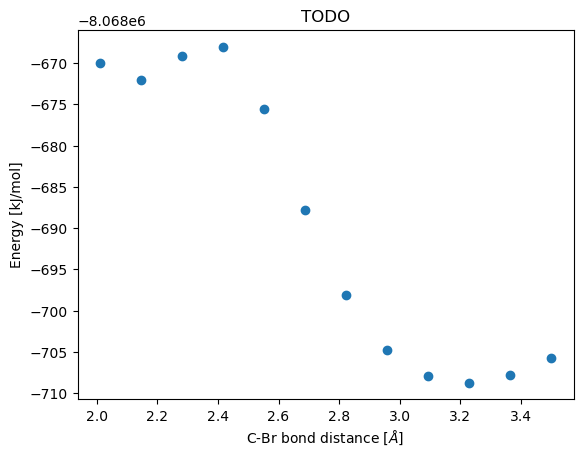
\includegraphics[width=0.8\textwidth]{pes_scan.png}
    \caption{Energy profile of the relaxed PES scan for the $S_N 2$ reaction. The transition state is indicated by the maximum at a carbon-bromine distance of approximately \SI{2.45}{\angstrom}.}
    \label{fig:pes_scan}
\end{figure}

The activation energy for the reaction was calculated to be approximately \SI{5.3}{kJ/mol}.
The vibrational mode corresponding to the imaginary frequency describes the motion along the reaction coordinate, which involves the simultaneous breaking of the carbon-bromine bond and the formation of the carbon-chlorine bond.

\subsection{Nudged Elastic Band (NEB) Calculation}

The NEB calculation provided a less detailed picture of the reaction pathway, since we used only five images in between the reactants and products. Still, the transition state was located at the fifth image, which corresponds to a different carbon-bromine distance of approximately \SI{3.2}{\angstrom}. This discrepancy leads to the different activation energy of approximately \SI{148.4}{kJ/mol} that we obtained from the NEB calculation, which is significantly higher than the value obtained from the relaxed PES scan.
The energy profile along the reaction coordinate showed a clear maximum at this point, indicating the presence of a transition state, which can be seen in figure \ref{fig:neb}.

\begin{figure}[H]
    \centering
    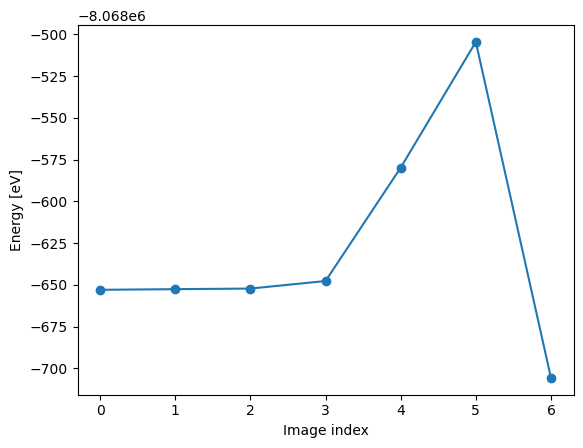
\includegraphics[width=0.8\textwidth]{neb.png}
    \caption{Energy profile of the NEB calculation for the $S_N 2$ reaction. The transition state is indicated by the maximum at the fifth image.}
    \label{fig:neb}
\end{figure}

\end{document}